\chapter{Introduction to Data Mining}
In the course of Data Mining are introduced and analyzed methods and models to use to analyze
large amount of data, so we start giving the definition of Data Mining as 
\begin{defi}
Data Mining is the use of efficient techniques for the analysis of very large collections of data and
the extraction of useful and possibly unexpected patterns in data (hidden knowledge)
\end{defi}
Enormous data growth in both commercial and scientific databases, due to advances in data generation and
collection technologies but also there is also a mantra that says to gather whatever data you can whenever and
wherever possible.

Lots of data is being collected and warehoused, like for example Web data, where Yahoo has Peta Bytes of web data
or also Facebook has billions of active users, also Amazon handles millions of visits each day and this also 
explains why know how to process and find useful information from huge amount of data will be very important.

Data are divided in two useful categories:
\begin{description}
    \item [Primary data: ] original data that has been collected for a specific purpose and they are 
                           not altered by humans.
    \item [Secondary data: ] data that has been already collected and made available for other purposes
                             and may be obtained from many sources.
\end{description}
The process of Knowledge discovered in database (KDD) can be described by figure \ref{img:phaseDataMining},
where we have input data that will have a preprocessing phase and then we applied to a data mining modelation
and we obtain the information gained.

\begin{figure}
    \caption{Phases on a Data Mining approach}
    \label{img:phaseDataMining}
    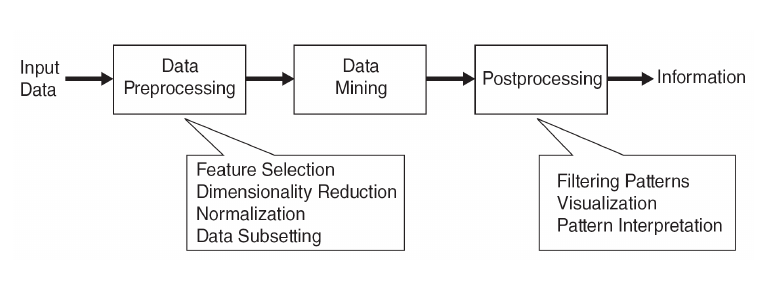
\includegraphics[width=\textwidth]{Images/dataMiningProcedure}
\end{figure}

We have so discovered that Data Mining is an phase of KDD process and we descrived all phases that can be 
viewed on \ref{img:kddProcess}, that will all analyzed during the course:
\begin{description}
    \item [Data Integration: ] involves the process of data understanding, data cleaning, merging data coming 
                               from multiple sources and transfoming them to load them
                               into a Data Warehouse Databases.
    \item [Data Warehouse: ]   is a database targeted to answer specific business questions.
    \item [Data Selection: ]   relevant data to analysis tasks are retrieved from data.
    \item [Data Transformation: ] transform data into appropriate form for mining (summary, aggregation, etc.)
    \item [Pattern Evaluation: ] Identify truly interesting patterns
    \item [Knowledge representation:] use visualization and knowledge representation tools to present
                                      the mined data to the user
\end{description}

\begin{figure}
    \caption{KDD process phases}
    \label{img:kddProcess}
    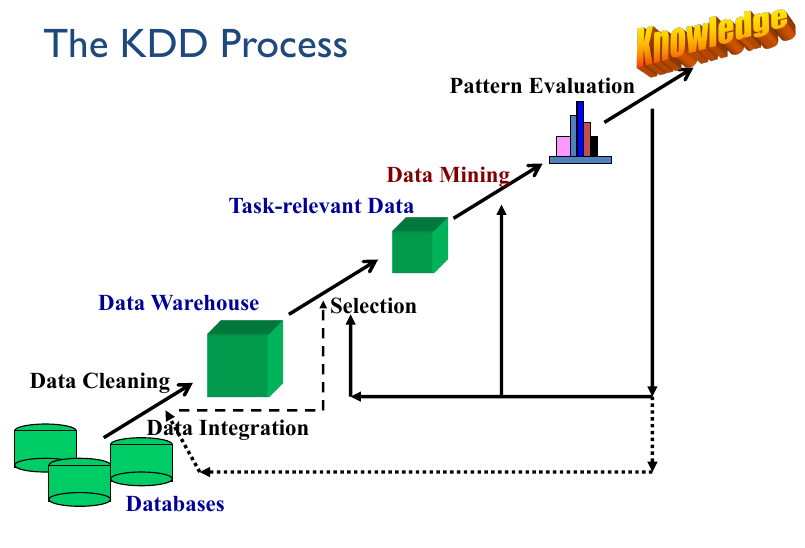
\includegraphics[width=\textwidth]{Images/kddProcess}
\end{figure}

Data Mining approches can be divided in two different tasks:
\begin{description}
    \item [Prediction Methods: ] we use some variables to predict unknown or future values of other variables.
    \item [Description Methods: ] the purpose is to find human-interpretable patterns that describe the data.
\end{description}
We now descrive the $4$ modellation task that are developed and used on Data Mining:
\begin{description}
    \item [Classification and Regression: ] refers to the task of building a model for the target variable
           as a function of explanatory variable and can be a \emph{classification} 
           (model for discrete class attribute) or a \emph{regression} where  we continuious data 
           where we would like to predict as a function of the values of other attributes.
    \item [Clustering: ] finding groups of objects such that the objects in a group will be similar (or related)
                         to one another and different from (or unrelated to) the objects in other groups.
    \item [Association Rules: ] Given a set of records each of which contain some number of items 
           from a given collection, produce dependency rules which will predict occurrence of an item based
           on occurrences of other items.\newline
           It is used in Market-basket analysis to optimize sales promotion and also in medical informatics to 
           find combination of patient symptoms and test results associated with certain diseases.
    \item [Anomaly Detection: ] detect significant deviations from normal behavior and it can be used 
                                in Credit Card fraud detection or in detect network intrusions.
\end{description}
Traditional techniques have often encountered practical difficulties in meeting the challenges posed by
big data application in particular in scalability of peta/etabytes of data, in high dimension of attributes, 
in heterogeneous and complex data and also in ownership of data so this is why was introduced and also used
data mining approach.

